\documentclass{beamer}

\mode<presentation>{
 	\useoutertheme{infolines}
	\usetheme{Frankfurt}
}

\usepackage[brazil]{babel}
\usepackage[utf8]{inputenc}
\usepackage{indentfirst}
\usepackage{verbatim}
\usepackage{harvard}

\setbeamertemplate{navigation symbols}{}

\title[Título]{Título}

\author[Referência do autor]{Nome do autor}

\institute[IFRN]{
	Instituto Federal de Educação, Ciência e Tecnologia do Rio Grande do Norte\\
	Nome do curso\\
	Nome do campus
}
  
\date[\today]{\today}

\begin{document}

\logo{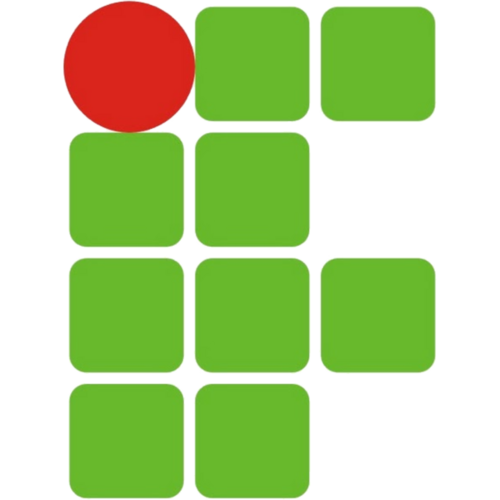
\includegraphics[scale=0.1]{imagens/IFRN}}

\begin{frame}[plain]
	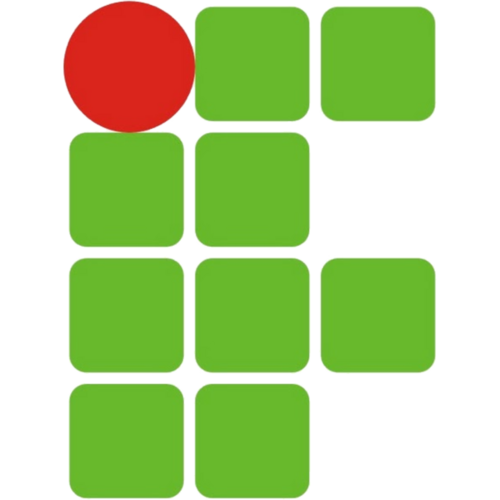
\includegraphics[scale=0.2]{imagens/IFRN}
	\titlepage
\end{frame}

\begin{frame}
	\frametitle{Sumário}
  	\tableofcontents
\end{frame}

\AtBeginSection[]{
	\begin{frame}
		\frametitle{Sumário}
		\tableofcontents[currentsection]
	\end{frame}
}

\section{Introdução}
\subsection*{}

\begin{frame}
	\frametitle{Problemática}

	\begin{itemize}
		\item
		\item
		\item
	\end{itemize}
\end{frame}

\begin{frame}
	\frametitle{Objetivos}

	\begin{itemize}
		\item
		\item
		\item
	\end{itemize}
\end{frame}

\begin{frame}
	\frametitle{Justificativas}

	\begin{itemize}
		\item
		\item
		\item
	\end{itemize}
\end{frame}

\section{Desenvolvimento}
\subsection*{}

\begin{frame}
	\frametitle{Desenvolvimento}

	\begin{itemize}
		\item
		\item
		\item
	\end{itemize}
\end{frame}

\section{Metodologia}
\subsection*{}

\begin{frame}
	\frametitle{Metodologia}

	\begin{itemize}
		\item
		\item
		\item
	\end{itemize}
\end{frame}

\section{Resultados}
\subsection*{}

\begin{frame}
	\frametitle{Resultados}

	\begin{itemize}
		\item
		\item
		\item
	\end{itemize}
\end{frame}

\section{Conclusão}
\subsection*{}

\begin{frame}
	\frametitle{Conclusões}

	\begin{itemize}
		\item
		\item
		\item
	\end{itemize}
\end{frame}

\begin{frame}
	\frametitle{Trabalhos Futuros}

	\begin{itemize}
		\item
		\item
		\item
	\end{itemize}
\end{frame}

\end{document}